%!TEX root = bambi-thesis.tex
This chapter begins with a theory digression about the topic of Coverage Path Planning. Then the algorithm chosen for the application in this thesis is explained in details and finally the ROS implementation of the algorithm is presented and discussed.
\section{Theory Background} % (fold)
\label{sec:theory_background}
\textit{Coverage path planning} (CPP) is the problem of finding a trajectory for a mobile robot such that a target area is completely swept by the sensor footprint. In the following section it is first presented the conventional CPP algorithms in use for mobile robots. Later, the focus moves more specifically over aerial application showing some previous work regarding this topic.

\subsection{Coverage Path Planning for Mobile Robots} % (fold)
\label{sub:coverage_path_planning_for_mobile_robots}
The problem of finding an optimal coverage path, even for a simple polygon, is classified as NP-hard \footnote{NP-hard problems are problems for which there is no known polynomial algorithm, so that the time to find a solution grows exponentially with problem size. Although it has not been definitively proven that, there is no polynomial algorithm for solving NP-hard problems, many eminent mathematicians have tried and failed.} \cite{ARKIN200025}. Hence, existing approaches try to find an approximate solution which fits at best the specific application requirements. For 2D coverage, some methods decompose the target area into simpler polygons and for each compute the coverage path. Other methods use a grid-based representation which leads to an approximate coverage. Finally, closed-loop control methods avoid the needs of an a priori representation of the target region.

\subsubsection{Exact Cellular Decomposition} % (fold)
\label{ssub:exact_cellular_decomposition}
One of the main approach in area coverage path planning is based on the divide-and-conquer strategy.
In this method the target area is decomposed in simple regions called cells. Since all cells have a simple structure, each can be covered with simple motions such as back-and-forth motion as in \autoref{fig:lawnmower-pattern}. This kind of motion is called \textit{Lawnmower pattern}. Once the robot visits all cell, coverage is achieved.\\
\textit{Trapezoidal decomposition} is the most popular cell decomposition. This decomposition relies heavily on the polygonal representation of the planar configuration space \cite{book:655068}. Cells are in fact obtained simply by sweeping a vertical line through the 2D plane and, upon reaching each vertex of the environment polygon, the required edges are added to create trapezoids (see \autoref{fig:trapezoidal-decomposition}). Two cells sharing a common boundary are defined as adjacent and accordingly an adjacent graph is produced. At this point the strategy consist in finding the exhaustive walk which visits all cells and minimizes the cost of traveling between them.
An important factor in finding an efficient path is the choice of the swiping direction line when decomposing the target area as analyze by Oksane \cite{TrapezoidalDecompCPP}. He performed a local optimization to find the direction for the sweeping line which minimize trajectory length and the number of turnings.
\begin{figure}[ht]
    \centering
    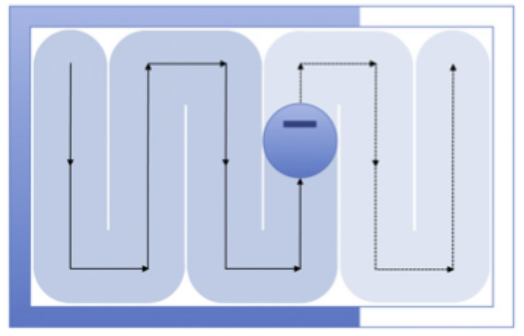
\includegraphics[width=0.4\textwidth]{figures/C3/LawnmowerPattern.png}
    \caption{Lawnmower pattern}
    \label{fig:lawnmower-pattern}
\end{figure}

\begin{figure}[ht]
    \centering
    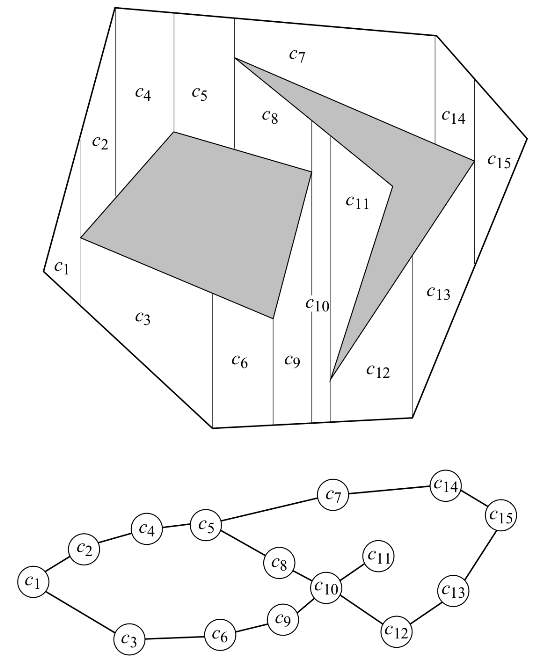
\includegraphics[width=0.5\textwidth]{figures/C3/TrapezoidalDecomposition.png}
    \caption{Trapezoidal decomposition and adjacent graph \cite{book:655068}}
    \label{fig:trapezoidal-decomposition}
\end{figure}
% subsubsection exact_cellular_decomposition (end)



% subsection coverage_path_planning_for_mobile_robots (end)
\subsection{Aerial Coverage using UAVs} % (fold)
\label{sub:aerial_coverage_using_uavs}


% The general CPP methods introduced in Chapter 2.2.1 have been applied directly to aerial coverage often in an offline setting. In these works, the target area is specified as a polygon or grid with GPS coordinates of the polygon nodes or grid center. It is usually assumed that the UAV is flying at an altitude which is safe and hence there is no risk of colliding with an obstacle. However sometimes some parts of the environment are treated as no-flying zones which should be avoided by the UAV. Therefore in CPP for UAVs, these subregions are dealt with as obstacles. Another type of region that might be present in aerial coverage is uninteresting regions. Flying in these regions is allowed but does not contribute to the coverage goal i.e. covering them is of no value. For example in a outdoor crop mapping task with a quadrotor, covering the lake is unnecessary but flying over it (for example to reach the other side of the lake) is allowed.\\
% As mentioned before, due to the very short flight time of UAVs, generating efficient coverage paths is useful. To reach efficiency, existing methods try to avoid unnecessary coverage, i.e. they try to minimize the overlap in the sensor footprint along the produced trajectory. This goal will consequently reduce the path length. Another element considered by some existing methods is to minimize the number of turns in the flight trajectory. Reducing the number of turnings will consequently produce trajectories that consist of long straight stripes, as is the case in Lawnmower pattern. Therefore, when a robot follows the trajectory it can maintain a constant velocity in a large part of the coverage path and it only accelerates or de-accelerates when it is turning. The overall outcome is less power consumption. Such efficient coverage trajectories can be planned offline when the environment is known a priori. Some of these methods, aimed for aerial coverage, are presented in the following section which includes planning for both single and multi-robot systems. However, when no prior knowledge about the target area is available, the planning has to be done online based on the real-time sensory data.\\
% In the following, we present the existing methods of coverage trajectories planning for unmanned aerial vehicles. We partition the approaches into two main groups: a) methods that precompute the trajectory based on a priori knowledge of the environment and b) methods that adaptively re-plan the trajectory based on on-line sensory data.
 % subsection aerial_coverage_using_uavs (end)

\subsection{Flight Altitude} % (fold)
\label{sub:flight_altitude}
How to compute the required flight altitude (resolution + sensor footprint + required photo overlap). Some calculation will be listed.
% subsection flight_altitude (end


% section theory_background (end)

\section{Proposal Solution} % (fold)
\label{sec:proposal_solution}

Abbiamo scelto il wavefront perche' oltre ad essere abbastanza efficente computazionalmente permette di tenere conto di diverse cost function (diverse priorita' come ad esempio l'altitudine, minor number of turns, ecc...)]
% section proposal_solution (end)


\section{Implementation in ROS} % (fold)
\label{sec:implementation_in_ros}


% section cpp_algorithms (end)